\documentclass[11pt]{scrartcl}
\usepackage[parfill]{parskip}
\usepackage{graphicx}
\usepackage{booktabs}
\usepackage{tabulary}
\usepackage{float}
\usepackage{hyperref}

\graphicspath{{../images/}}

\title{\textbf{Case Studies II - Community Talks}}
\subtitle{Technologies and Contributions}
\author{Ricardo Garc\'ia Fern\'andez}
\date{\today}

\begin{document}

\maketitle

\vfill

\begin{flushright}
    \copyright  2013 Ricardo Garc\'ia Fern\'andez - ricardogarfe [at] gmail [dot] com.

    This work is licensed under a Creative Commons 3.0 Unported License.
    To view a copy of this license visit:
 
    \url{http://creativecommons.org/licenses/by/3.0/legalcode}.
\end{flushright}

\begin{figure}[h]
    \begin{flushright}	
        
\includegraphics{by}
        \label{fig:by}
    \end{flushright}
\end{figure}

\newpage

\tableofcontents

\newpage

\section{Thunderbird Q\&A}
\label{sec:thunderbird-qa}

\begin{figure}[H]
\centering

\includegraphics[width=\textwidth]{mozilla-thunderbird.png}   
\caption{Thunderbird Community Talk by \href{https://twitter.com/lhirlimann}{\emph{Ludovic Hirliman}}}
\label{thunderbird}
\end{figure}

\par \href{http://www.mozilla.org/es-ES/thunderbird/}{Thunderbird} is a FLOSS Email client from Mozilla Foundation \textit{- MOFO -} . Latest news aren't good news because Mozilla stop development resources to this project on July 2012\footnote{Thunderbird finale - \url{https://blog.lizardwrangler.com/2012/07/06/thunderbird-stability-and-community-innovation/}} but this talk showed us the way developers work in Thunderbird and how Quality \& Assurance \textit{- Q\&A -} Team and developers join efforts to lead a better development.

\par Ludovic Hirliman\footnote{Ludovic Hirliman web - \url{http://perso.hirlimann.net/~ludo/}} is\textit{Q\&A}leader in Thunderbird, through his vision we are capable of see the big picture behind good software development starting with Test Driven Development \textit{- TDD -} .

\begin{center}
    \textit{"Testing Tools: your hand, your brain and time" by Ludovic Hirliman.}
\end{center}

\subsection{Development Tools} "Someone wants to test ? go to url, test and report bugs"Focusing in our goals, here are Thunderbird development tools:
\begin{itemize}
	\item \textit{Bug Tracking Sustem} - Bugzilla - Everyone could post a bug and how to replicate a bug there.
	\item \textit{Test case management software} - \href{https://mail.mozilla.org/pipermail/thunderbird-testers/2012-October/000111.html}{From Litmus to Moztrap}. Tools to create and run test cases related to email clients.
\begin{itemize}
	\item \href{http://litmus.com/}{Limus} - Test interactively with real email clients.
	\item \href{http://moztrap.wordpress.com/}{Moztrap} - Test Case Management from Mozilla.
\end{itemize}
	\item \textit{Continuous Integration} - \href{http://trac.buildbot.net/}{Buildbot} - Checkout, run make, run make test, read log file and automate a build in every commit. Running unit test to build after each commit.
	\item \textit{Documentation} - Wiki to develop extensions and a real user Wiki.
	\item \textit{Communication} - IRC as main communication channel, group chats, history in\#tb-support-crew.
	\item \textit{Testing Tool} - \href{http://docs.seleniumhq.org/}{Selenium} - Framework to automate integration browser testing.
\end{itemize} After throw away all spaghetti code in 2009, next QA goal in January 2010 was: "To add code to Thunderbird developers have to develop tests". After those steps the project obtain more volunteers. The code you write matters and its easy to contribute, collaborate and test.

\begin{figure}[H]
\centering
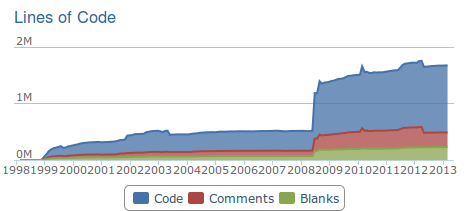
\includegraphics[width=0.7\textwidth]{thunderbird-code-evolution.png}
\caption{Thunderbird code evolution}
\label{}
\end{figure}

Thunderbird lines of code evolution jumps in 2009, filled with test classes

\subsection{How to Contribute}

There are many ways to contribute to Thunderbird, be a user is the first step to dive into the community:

\begin{itemize}
	\item \textit{Development} - Reporting bugs, patches and contributing with code.
	\item \textit{Q\&A} - After failling Mozilla\href{https://quality.mozilla.org/2013/03/mozilla-org-test-day/}{Friday test day}process into Thunderbird community, they changed the question to: \textit{"Do you want to contribute with test ?"} Thus they manage people and explain what and how they 'have to' test. Its an easier way to start to collaborate instead of \textit{"Someone wants to test ? go to url, test and report bugs"}. Better and easy as human way.
	\item \textit{Support} - Translations and localizations.
	\item \textit{Marketing} - Mozilla products Evangelist. Spreading the goods and benefits of MOFO products.
	\item \textit{Superheroes} - Thunderbird Contributors \href{https://support.mozillamessaging.com/es/kb/buscamos-superhroes}{starting page}inmozillamessaging.
	\item \textit{Forum} - Thunderbird \href{https://getsatisfaction.com/mozilla_messaging/}{forum} to search and generate information.
\end{itemize}
% section thunderbird-qa (end)

\begin{thebibliography}{9}

    \bibitem{thunderbird-talk}
    Thunderbird Community Talk,\\
    Ludovic Hirliman,\\  
    Part 1,\\
    \url{http://blip.tv/mswl/case-studie-ii_quality-assurance-in-thunderbird-and-mozilla-5906218},\\
    Part 2 Questions and Answers,\\
    \url{http://blip.tv/mswl/case-studie-ii_quality-assurance-in-thunderbird-and-mozilla-5906218}

\end{thebibliography}

\end{document}

